\documentclass{thesis-SJ}
\usepackage{amsmath}
\usepackage{amsthm}
\usepackage{amssymb}
\usepackage{mathtools}
\usepackage{physics}
\usepackage{graphicx}
\usepackage{caption}
\usepackage{hyperref} 
\usepackage{listings}


\usepackage{color}
\definecolor{mygreen}{RGB}{28,172,0}
\definecolor{mylilas}{RGB}{170,55,241}



\renewcommand{\figurename}{그림}
\renewcommand{\tablename}{표}

\title[Simulating Einstein’s Special Relativity Using R Tilde Matrix and MATLAB]{R Tilde 행렬과 MATLAB을 이용한 아인슈타인의 특수 상대성이론 시뮬레이션 구현}

\authorone[崔晸譚]{최정담}{Choi, Jung Dam} 
\studentnumberone{2214}

\authortwo[辛柱衡]{신주형}{Shin, Ju Hyeong} 
\studentnumbertwo{2308}

\advisor{권현우}{Hyunwoo Kwon}
\teacher{이예찬}{Yechan Lee}
\referee[1]{이순신}
\referee[2]{권율}

\date{2018년 11월 21일}{November 21st, 2018}

%\title[Test]{논문제목}
%\author{Hong, Gil Dong} 

\begin{document}

\KoreanAbstract

본 연구에서는 아인슈타인의 특수 상대성 이론, 즉 로렌츠 변환을 해석하며 R Tilde 행렬이라는 개념을 도입하였고, 이 행렬의 다양한 수학적인 성질들을 확인해 보았다. 또 본 연구에서는 R Tilde 행렬을 통한 선형변환을 원, 쌍곡선 등의 다양한 물리적(기하학적인) 상황에 적용하여 그 수학적 의미를 파악해보고자 하였다. 이후에는 행렬 연산에 특화되어 있는 MATLAB이라는 프로그램에 R Tilde 행렬을 활용하여, 특수 상대성이론 시뮬레이션을 제작하였으며, 특수 상대성이론을 학습하는 데 도움이 될 수 있도록 GUI 형태로 이를 변환하였다.

\KoreanKeywords{R Tilde, 특수 상대성이론, 로렌츠 변환, MATLAB, 시뮬레이션}

\tableofcontents
 
\mainpartstart

\chapter{서론} 

1905년 아인슈타인은 빛의 속도에 가깝게 움직이는 물체들에 대하여 모든 관성계는 동등하고, 모든 관성계에서 진공에서의 빛의 속력은 어디에서나 일정하다는 두 가지 가정을 통하여 특수 상대성이론이라는 새로운 물리 법칙을 제안하였다. 특수 상대성이론의 핵심적인 내용은 모든 좌표계에서 빛의 속력을 일정하게 유지시키기 위해 좌표계의 시간 축과 공간 축이 변화하여야 한다는 내용인데, 이는 빛의 속력에 근접하지 않은 관측자에서는 유의미하게 드러나지 않으므로 일상적인 상황에서는 특수 상대론적인 효과가 잘 드러나지 않고, 그러므로 특수 상대성이론을 직관적으로 이해하는 것은 어려운 편이다. 

한편 민코스프키는 민코스프키 기하학이라는 새로운 비유클리드 기하학을 창시하여 아인슈타인의 특수 상대성이론을 수학적으로 해석하고자 하였다. 민코스프키 기하학의 한 가지 특징은 모든 축(시간 축 및 공간 축)이 서로 직교하나 민코스프기 기하 위의 두 좌표 사이의 거리가 식 \eqref{dist} 과 같이 주어진다는 것이다. 식 \eqref{dist}는 $(\Delta t)^2$의 부호가 음수라는 것에서 일반적인 유클리드 기하학에서의 두 점 사이의 거리와 차이를 보인다.

\begin{equation}
	(\Delta s)^2 = (\Delta x)^2 + (\Delta y)^2 + (\Delta z)^2 - (\Delta t)^2 \label{dist}
\end{equation}

민코스프키는 이후 아인슈타인의 특수 상대성이론이 민코스프키 시공간의 좌표 변환이라는 사실을 발견하고, 이 좌표 변환이 두 점 사이의 거리 $(\Delta s)^2$를 변화시키지 않는다는 사실을 알아내었다. 이를 직관적으로 이해할 수 있게 만든 것이 민코스프키 다이어그램, 혹은 민코스프키 시공도식이다. 이는 직관적일 뿐더러, 특수 상대성이론의 물리적 의미가 잘 담겨 있으나, 손으로 민코스프키 시공도식을 그리는 것이 비교적 어렵다는 단점이 있다. 따라서 본 연구는 이러한 민코스프키 시공도식의 강점을 살리면서도, 다양한 물리적 상황에 대하여 쉽게 민코스프키 시공 도식을 작성하고 특수 상대론의 물리적 의미를 이해할 수 있도록 특수 상대성이론 시뮬레이션을 제작하는 데에 주목하였다. 이 과정에서 특수 상대성 이론을 민코스프키 시공간의 좌표축 변환으로 해석하는 민코스프키의 아이디어에 주목하여 시공간 축의 변환을 선형 변환으로 해석하고자 하였고, 이에 R Tilde 행렬을 도입하였다.

\chapter{이론적 배경}

\section{특수 상대성이론}
특수 상대성이론은 1905년 아인슈타인이 발표한 개념으로, 등속도로 움직이는 서로 다른 두 좌표계의 물리량 사이의 관계를 표현하고 있다. 특히 이 관계는 로렌츠 변환이라는 네 개의 등식에 의하여 표현된다. 관성계 $S$에서 본 사건의 좌표를 $(t,x,y,z)$, 관성계 $S'$에서 본 사건의 좌표를 $(t', x',y',z')$라 하면, 서로 다른 두 좌표계에서 본 사건 $E$, $E'$가 $E(0,0,0,0)=E'(0,0,0,0)$를 만족할 때 다음과 같은 식이 성립한다.

\begin{equation}
\begin{gathered}
t' = \gamma(t-\frac{ux}{c^2}) \\
x' = \gamma(x-ut) \\
y' = y \\
z' = z
\end{gathered} \label{lorentz}
\end{equation}
 
단, 식 \eqref{lorentz}에서 $\mathbf{u}$는 관성계 $S$에서 본 관성계 $S'$의 속도이며, $u=\abs{\mathbf{u}}$이다. 한편 $\gamma$는 다음과 같이 정의된다.

\begin{equation*}
	\gamma = \frac{1}{\sqrt{1-u^2/c^2}}
\end{equation*} 

한편 민코프스키 시공간에서, 시공간 좌표는 다음과 같이 벡터로 표현할 수 있다.

\begin{equation}
	\vec{E} = \begin{pmatrix}
	t \\ x \\ y \\ z
	\end{pmatrix}
\end{equation}

그렇게 했을 때, 식 \eqref{lorentz}는 다음과 같이 표현할 수 있다.
\begin{equation}
	\begin{gathered}
	\vec{E'}=L\vec{E}
	\\
    \text{where} \\
	L = \begin{pmatrix}
	\gamma & -u\gamma & 0 & 0 \\
	-u\gamma & \gamma & 0 & 0 \\
	0 & 0 & 1 & 0 \\
	0 & 0 & 0 & 1
	\end{pmatrix}
	\end{gathered} \label{lorentzmat}
\end{equation}

이것이 민코스프키 시공간을 통해 표현한 로렌츠 변환 행렬식이다.

\section{오일러 회전 변환 행렬}

어떤 점 $\vec{P} = \begin{pmatrix}
x\\y
\end{pmatrix}$를 반시계방향으로 $\theta$만큼 돌린 점을 $\vec{P} = \begin{pmatrix}
x'\\y'
\end{pmatrix}$라고 하자. 이 때 $\vec{P}$와 $\vec{P'}$ 사이에는 다음과 같은 관계가 있다.

\begin{equation}
\begin{gathered}
\vec{P'}=R_\theta \vec{P} \\
\text{where} \\
R_\theta = \begin{pmatrix}
\cos \theta & \sin \theta \\
-\sin \theta & \cos \theta 
\end{pmatrix}
\end{gathered}
\end{equation}

이 때 $R_\theta$는 다음과 같은 성질을 가지고 있다.

\begin{enumerate}
	\item 크기 보존; 어떤 도형에 $R_\theta$를 적용한 후의 도형도 원래 도형과 그 크기가 동일하다. 즉,
	
	\begin{equation}
		\det(R_\theta) = 1
	\end{equation}
	
	\begin{proof}
		
		\begin{align*}
			& \det(R_\theta) \\
			&= \det\begin{pmatrix}
			\cos \theta & \sin \theta \\
			-\sin \theta & \cos \theta 
			\end{pmatrix} \\
			&= \cos^2\theta +\sin^2\theta \\
			&= 1
		\end{align*}
	\end{proof}
	
	\item Homomorphism; $\theta_1+\theta_2$만큼 회전시키는 회전 행렬과 $\theta_1$과 $\theta_2$를 회전시키는 회전 행렬을 각각 수행한 회전 행렬은 같다. 즉,
	
	\begin{equation}
		R_{\theta_1} R_{\theta_2} =R_{\theta_1+\theta_2}
	\end{equation}
	
	\begin{proof}
		\begin{align*}
		& R_{\theta_1} R_{\theta_2} \\
		&= \begin{pmatrix}
		\cos \theta_1 & \sin \theta_1 \\
		-\sin \theta_1 & \cos \theta_1 
		\end{pmatrix}\begin{pmatrix}
		\cos \theta_2 & \sin \theta_2 \\
		-\sin \theta_2 & \cos \theta_2
		\end{pmatrix}\\
		&=\begin{pmatrix}
		\cos \theta_1\cos \theta_2 - \sin \theta_1\sin \theta_2& \cos \theta_1\sin \theta_2 + \sin \theta_1\cos \theta_2\\
	 -\sin \theta_1\cos \theta_2+\cos \theta_1(-\sin \theta_2)& 	-\sin \theta_1\sin \theta_2 + \cos \theta_1\cos \theta_2
		\end{pmatrix}\\
		&=\begin{pmatrix}
		\cos (\theta_1+\theta_2) & \sin (\theta_1+\theta_2) \\
		-\sin (\theta_1+\theta_2) & \cos (\theta_1+\theta_2)
		\end{pmatrix}\\
		&= R_{\theta_1+\theta_2}
		\end{align*}
	\end{proof}
\end{enumerate}

한 편 3차원 좌표에서 xy 축으로 회전하는 오일러 회전 행렬은 다음과 같이 표현할 수 있다.

\begin{equation}
	R_\theta = \begin{pmatrix}
	\cos \theta & \sin \theta & 0\\
	-\sin \theta & \cos \theta & 0 \\
	0 & 0 & 1
	\end{pmatrix}
\end{equation}

이를 $n$차 민코스프키 시공도식까지 확장하면 다음과 같다.

\begin{equation}
R_\theta = \underbrace{\begin{pmatrix}
\cos \theta & \sin \theta & 0 & 0 & \cdots & 0\\
-\sin \theta & \cos \theta & 0 & 0 & \cdots & 0\\
0 & 0 & 1 & 0 & \cdots & 0 \\
0 & 0 & 0 & 1 & \cdots & 0 \\
\vdots & \vdots & \vdots & \vdots & \ddots & \vdots \\
0 & 0 & 0 & 0& 0 & 1
\end{pmatrix}}_{n \text{ elements}}
\end{equation}
\section{민코스프키 시공도식}

민코스프키 시공도식은 특수 상대성이론을 시각화하기 위해 만든 도식으로, 다음과 같은 규칙으로 작성한다.

\begin{enumerate}
	\item $x$축에는 $\mathbf{u}$의 방향과 같은 축의 위치 축을, $y$축에는 $ct$ 축을 기입한다. 그러므로 빛의 이동 경로는 언제나 $x$축과 $\pm\frac{\pi}{4}$의 각을 이룬다.
	\item 로렌츠 변환은 시간 축과 공간 축을 회전시킴으로써 이루어진다. 이 때 회전 각도는 $\tan^{-1}(\frac{v}{c})$이며, 공간 축은 반시계 방향으로, 시간 축은 시계 방향으로 회전한다.
	\item 좌표의 스케일 역시 바뀐다. 이 때, 서로 다른 좌표축에서의, 좌표가 $(k,0)$인 서로 다른 점들의 모임은 $x^2-t^2=k^2$을 만족하는 쌍곡선 위에 있다.\footnote{식 \eqref{dist}를 참고하여라.} 한 편 서로 다른 좌표축에서의 좌표가 $(0,l)$인 서로 다른 점들의 모임은 $t^2-x^2=l^2$을 만족시킨다.
\end{enumerate}


그림 \ref{fig:diagram}는 이러한 규칙으로 작성한 민코스프키 시공도식의 예이다.

\begin{figure}[h]
	\centering
	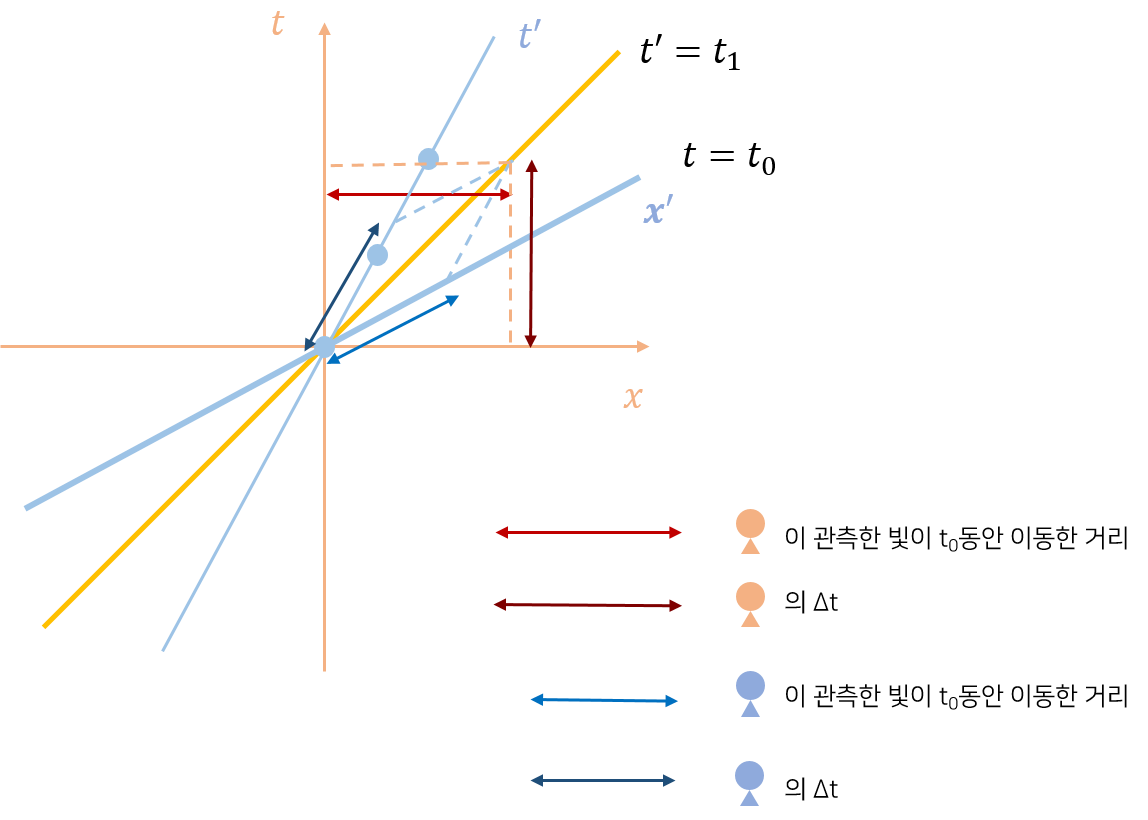
\includegraphics[width=0.5\linewidth]{images/diagram}
	\captionof{figure}{민코스프키 시공도식}
	\label{fig:diagram}
\end{figure}

\chapter{연구 결과}
\section{R Tilde 행렬}
\subsection{R Tilde 행렬의 정의와 성질}
$2$차원 상에서의 R Tilde 행렬을 다음과 같이 정의한다.

\begin{equation}
	\tilde{R}_\theta = \begin{pmatrix}
	\cosh \theta & -\sinh \theta \\
	-\sinh \theta & \cosh \theta 
	\end{pmatrix}
\end{equation}

이 때 R Tilde 행렬은 오일러 행렬과 다음과 같은 공통점을 가진다.

\begin{enumerate}
	\item 크기 보존; 어떤 도형에 $\tilde{R}_\theta$를 적용한 후의 도형도 원래 도형과 그 크기가 동일하다. 즉,
	
	\begin{equation}
	\det(\tilde{R}_\theta) = 1
	\end{equation}
	
	\begin{proof}
		
		\begin{align*}
		&\det(\tilde{R}_\theta)\\
		&=\det\begin{pmatrix}
		\cosh \theta & -\sinh \theta \\
		-\sinh \theta & \cosh \theta 
		\end{pmatrix}\\
		&= \cosh^2{\theta} - \sinh^2{\theta} \\
		&= 1
		\end{align*}
	\end{proof}
	
	\item Homomorphism; $\theta_1+\theta_2$만큼 회전시키는 R tilde 행렬과 $\theta_1$과 $\theta_2$를 회전시키는 R tilde 행렬을 각각 수행한 회전 행렬은 같다. 즉,
	
	\begin{equation}
	\tilde{R}_{\theta_1}\tilde{R}_{\theta_2} =\tilde{R}_{\theta_1+\theta_2}
	\end{equation}
	
	\begin{proof}
		$\tilde{R}_\theta$의 대각화부터 시작한다.
		
		 \begin{align*}
		\det(\tilde{R}-\lambda I) &= 0 \\
		(\cosh{x}-\lambda)^2-\sinh^2{x} &= 0 \\
		(\cosh{x}-\lambda)&=\pm \sinh{x}
		\end{align*}
		
		 \begin{align*}
		\lambda &= \cosh{x} \pm \sinh{x} \\
		&= e^x \quad \text{or} \quad e^{-x}
		\end{align*}
		
		 \begin{equation}
		\tilde{R}_\theta = \left(\frac{1}{\sqrt{2}}\begin{pmatrix}
		1 & 1 \\ -1 & 1
		\end{pmatrix}\right) \begin{pmatrix}
		0 & e^\theta \\ e^{-\theta} & 0
		\end{pmatrix} \left(\frac{1}{\sqrt{2}}\begin{pmatrix}
		-1 & -1 \\ 1 & -1
		\end{pmatrix}\right)
		\end{equation}

	\begin{align*}
	\tilde{R}_{\theta_1}\cross \tilde{R}_{\theta_2} &= \left(\frac{1}{\sqrt{2}}\begin{pmatrix}
	1 & 1 \\ -1 & 1
	\end{pmatrix}\right) \begin{pmatrix}
	0 & e^{\theta_1+\theta_2} \\ e^{-({\theta_1+\theta_2})} & 0
	\end{pmatrix} \left(\frac{1}{\sqrt{2}}\begin{pmatrix}
	-1 & -1 \\ 1 & -1
	\end{pmatrix}\right) \\
	&= \tilde{R}_{(\theta_1+\theta_2)}
	\end{align*}
	
	
\end{proof}

\end{enumerate}

즉, $\cosh \theta$와 $\sinh \theta$로 이루어진 $\tilde{R}_\theta$는 $R_\theta$와 같은 성질을 보인다. 이 성질을 유지하도록 $\tilde{R}_\theta$를 $n$차까지 확장하면 이는 다음과 같다.

\begin{equation}
\tilde{R}_\theta = \underbrace{\begin{pmatrix}
	\cosh \theta & -\sinh \theta & 0 & 0 & \cdots & 0\\
	-\sinh \theta & \cosh \theta & 0 & 0 & \cdots & 0\\
	0 & 0 & 1 & 0 & \cdots & 0 \\
	0 & 0 & 0 & 1 & \cdots & 0 \\
	\vdots & \vdots & \vdots & \vdots & \ddots & \vdots \\
	0 & 0 & 0 & 0& 0 & 1
	\end{pmatrix}}_{n \text{ elements}}
\end{equation}

 R Tilde 행렬은 $\theta<0$일 때 x축과 y축을 회전시키되, x축은 반시계방향으로, y축은 시계방향으로 회전시킨다. 이 때 회전 각도는 R Tilde 행렬의 기하적인 의미는 hyperbolic angle의 기하적 의미를 통해 알아낼 수 있다. 원래 x 좌표축에서부터 회전한 x 좌표축 까지 $x^2-y^2=1$의 단위 쌍곡선을 타고 쓸어간 넓이는 정확히 $\frac{\theta}{2}$가 된다. 이는 오일러 회전 행렬에서의 $\theta$의 의미와 공통점이 있는데, 오일러 회전 행렬으로 원래 x 좌표축에서부터 회전한 x 좌표축까지 단위원을 타고 쓸어간 넓이 역시 정확히 $\frac{\theta}{2}$가 되기 때문이다.
 
\subsection{다양한 곡선의 R Tilde 회전 변환}

본 부분부터는 R Tilde 회전 변환에서 $\theta<0$인 경우를 다룰 것이다. 이 경우에는 $\theta$를 양수로 만들고 R Tilde 행렬을 다음과 같이 적용할 수 있다.

\begin{equation*}
\tilde{R}_\theta = \begin{pmatrix}
\cosh \theta & \sinh \theta \\
\sinh \theta & \cosh \theta 
\end{pmatrix}
\end{equation*}
\subsubsection{직선}
직선의 방정식은 일반적으로 $ax+by+c=0$을 만족한다. 이를 R Tilde 회전 변환시키면

\begin{align*}
\begin{pmatrix}
x' \\ y'
\end{pmatrix} &= \begin{pmatrix}\cosh{\theta} & \sinh{\theta} \\ \sinh{\theta} & \cosh{\theta} \end{pmatrix} \begin{pmatrix}
x \\ y
\end{pmatrix} \\
\begin{pmatrix}
x \\ y
\end{pmatrix} &=
\begin{pmatrix}
\cosh{\theta} & -\sinh{\theta} \\ -\sinh{\theta} & \cosh{\theta}
\end{pmatrix}  \begin{pmatrix}
x' \\ y'
\end{pmatrix} \\
&= \begin{pmatrix}
\cosh{\theta} x' - \sinh{\theta} y'\\ -\sinh{\theta} x' +\cosh{\theta} y'
\end{pmatrix}
\end{align*}

\begin{gather*}
ax + by + c = 0\\
\text{if}\phantom{a} a\neq \pm b\text{, wlog, }\\
\sinh{\theta_0} x + \cosh{\theta_0} y + c = 0 \\
\text{or}\\
\cosh{\theta_0} x + \sinh{\theta_0} y + c = 0
\end{gather*}

\begin{align*}
\cosh{\theta_0}(\cosh\theta x' - \sinh\theta y') + \sinh{\theta_0}(-\sinh{\theta} x' +\cosh{\theta} y')+c&=0\\
(\cosh{\theta_0}\cosh\theta- \sinh{\theta_0}\sinh{\theta})x'+(-\cosh{\theta_0}\sinh\theta+\sinh{\theta_0}\cosh{\theta} )y'+c&=0
\end{align*}

\begin{align*}
\sinh{\theta_0}(\cosh\theta x' - \sinh\theta y') + \cosh{\theta_0}(-\sinh{\theta} x' +\cosh{\theta} y')+c&=0\\
(\sinh{\theta_0}\cosh\theta- \cosh{\theta_0}\sinh{\theta})x'+(-\sinh{\theta_0}\sinh\theta+\cosh{\theta_0}\cosh{\theta} )y'+c&=0
\end{align*}
즉 직선을 R Tilde 회전시키면 직선의 hyperbolic angle이 $\theta$만큼 줄어들게 된다. 이는 오일러 회전 행렬과 동일한 결과이다.

\subsubsection{원}

$x^2+y^2=1$의 단위원을 생각하자. 이 원에 R Tilde 행렬을 적용하면 이는 $\frac{\pi}{4}$만큼 회전한 타원이 나온다.\footnote{$-\frac{\pi}{4}$만큼 회전했다는 것과 논리적으로 동치이다.}

\begin{align*}
\begin{pmatrix}
x' \\ y'
\end{pmatrix} &= \begin{pmatrix}\frac{1}{\sqrt{2}} & -\frac{1}{\sqrt{2}} \\ \frac{1}{\sqrt{2}} & \frac{1}{\sqrt{2}}\end{pmatrix} \begin{pmatrix}\cosh{\theta} & \sinh{\theta} \\ \sinh{\theta} & \cosh{\theta} \end{pmatrix} \begin{pmatrix}
x \\ y
\end{pmatrix} \\
\begin{pmatrix}
x \\ y
\end{pmatrix} &=
\begin{pmatrix}
\cosh{\theta} & -\sinh{\theta} \\ -\sinh{\theta} & \cosh{\theta}
\end{pmatrix} \begin{pmatrix}\frac{1}{\sqrt{2}} & \frac{1}{\sqrt{2}} \\ -\frac{1}{\sqrt{2}} &\frac{1}{\sqrt{2}} \end{pmatrix} \begin{pmatrix}
x' \\ y'
\end{pmatrix} \\
&= \begin{pmatrix}
x'\left(\frac{1}{\sqrt{2}}\cosh\theta +\frac{1}{\sqrt{2}}\sinh\theta\right)+y'\left(\frac{1}{\sqrt{2}}\cosh\theta -\frac{1}{\sqrt{2}}\sinh\theta\right)\\ y'\left(\frac{1}{\sqrt{2}}\cosh\theta -\frac{1}{\sqrt{2}}\sinh\theta\right)+x'\left(\frac{1}{\sqrt{2}}\cosh\theta +\frac{1}{\sqrt{2}}\sinh\theta\right)
\end{pmatrix}
\end{align*}

\[x^2+y^2=1\]

\begin{align*}
&\left\{x'\left(\frac{1}{\sqrt{2}}\cosh\theta +\frac{1}{\sqrt{2}}\sinh\theta\right)+y'\left(\frac{1}{\sqrt{2}}\cosh\theta -\frac{1}{\sqrt{2}}\sinh\theta\right)\right\}^2\\
&+\left\{y'\left(\frac{1}{\sqrt{2}}\cosh\theta -\frac{1}{\sqrt{2}}\sinh\theta\right)+x'\left(\frac{1}{\sqrt{2}}\cosh\theta +\frac{1}{\sqrt{2}}\sinh\theta\right)\right\}^2=1
\end{align*}

\[  x'^2(\cosh\theta+\sinh\theta)^2 + y'^2(\cosh\theta - \sinh\theta)^2=1\]

이 결과는 Geogebra로도 확인할 수 있었다.


\begin{figure}[h]
	\centering
	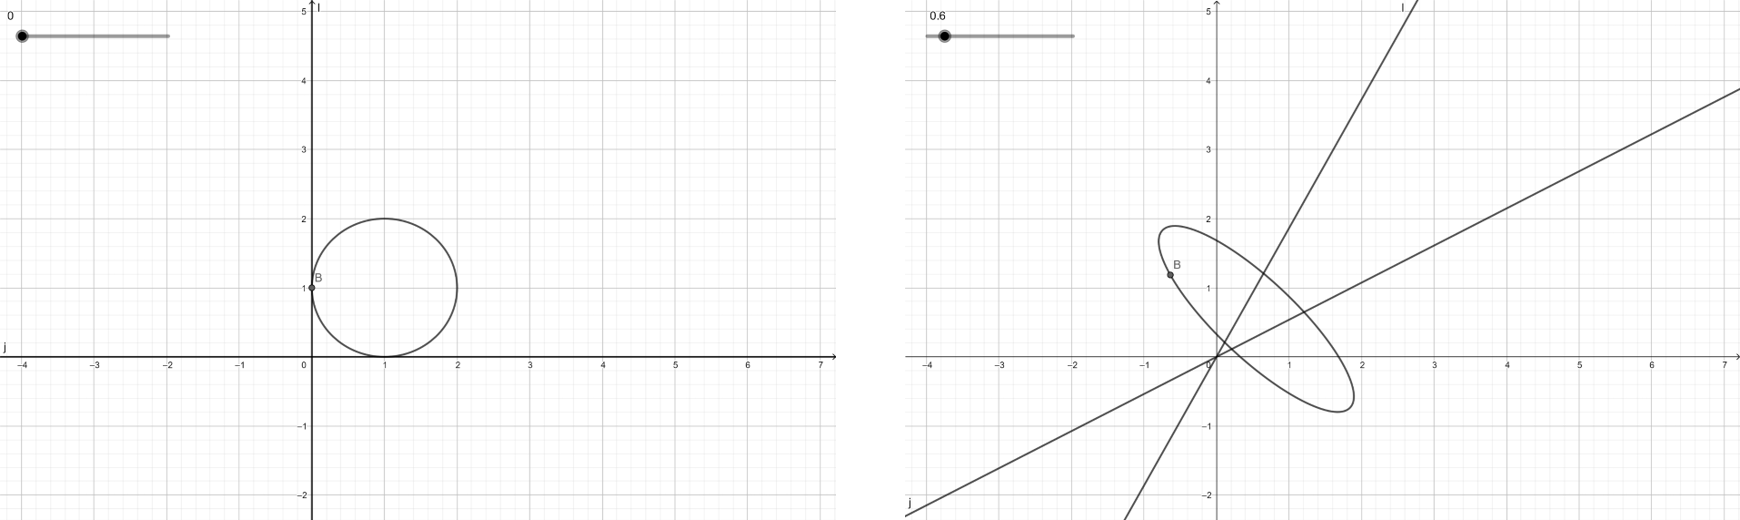
\includegraphics[width=0.7\linewidth]{images/geogebra}
	\caption{원의 R Tilde 회전, 우측 타원은 회전한 좌표축에서 본 원의 모습}
	\label{fig:geogebra}
\end{figure}

\subsubsection{쌍곡선}

단위 쌍곡선을 R Tilde 회전 변환하면 단위 쌍곡선이 나온다. 이는 단위 원을 오일러 회전 변환하면 단위 원이 된다는 사실과 연결된다.


\[  x^2-y^2=1 \]

\begin{align*}
(\cosh\theta x' -\sinh\theta y')^2 - (-\sinh\theta x' +\cosh \theta y')^2 &=1 \\
(\cosh^2\theta - \sinh^2\theta)x'^2 + (\sinh^2\theta - \cosh^2\theta)y'^2&=1
\end{align*}

\[  x'^2-y'^2=1 \]

\section{MATLAB 시뮬레이션}

\subsection{로렌츠 변환의 행렬 표현}
로렌츠 변환은 원점이 같고, $x$방향으로만 이동하는 관성계에 대해 식 \eqref{lorentzmat}으로 표현된다. 이를 R Tilde 행렬을 이용하여 표현하면 다음과 같다.

\begin{equation}
\begin{gathered}
L = \tilde{R}_\theta\\
\text{where} \\
\theta = \gamma
\end{gathered}
\end{equation}

한편 관성계의 원점을 맞추고, 관성계가 $x$축으로 움직이도록 하게 만들면 최종 식은 다음과 같아진다.

\begin{equation}
	O'_i = R_{\theta}\cross \tilde{R}_{\theta'}\cross R \cross (O_i - S)
\end{equation}

여기에서 각 행렬은 다음과 같다.

\[ S_{ij} = O_{i1} \]
\[ R_{\theta} = \begin{pmatrix}
1 & 0 & 0 \\
0 & \cos \theta & \sin \theta \\
0 & -\sin \theta & \cos \theta 
\end{pmatrix}\text{ where }\theta=\tan^{-1}\frac{v_y}{v_x} \] 

\[ \tilde{R}_{\theta'} = \begin{pmatrix}
\cosh \theta' & -\sinh \theta' & 0\\
-\sinh \theta' & \cosh \theta' & 0\\
0 & 0 & 1
\end{pmatrix} \text{ where } \theta' = \cosh^{-1} \gamma \]


\subsection{Text 기반 프로그램 작성 코드}
최종 목표를 달성하기 이전에 Text 기반으로 입출력을 받아 특수 상대성 이론을 시뮬레이션하는 프로그램을 제작하였다. 다양한 물체의 초기 위치, 속도, 아주 작은 크기의 가속도를 입력하면, 해당 물체들 중 하나를 기준으로 민코스프키 시공도식과 실제 물체 움직임을 애니메이션으로 출력하게 된다. 해당 프로그램의 실행 모습은 그림 \ref{fig:simulation}, \ref{fig:diagram}, \ref{fig:animation}과 같다.
\begin{figure}[h]
	\centering
	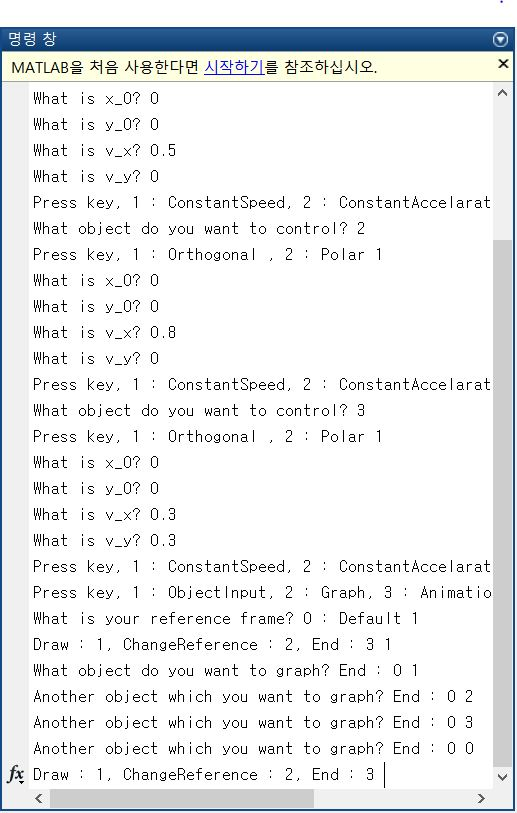
\includegraphics[width=0.6\linewidth]{images/simulation}
	\caption{Text 창}
	\label{fig:simulation}
\end{figure}

\begin{figure}[h]
	\centering
	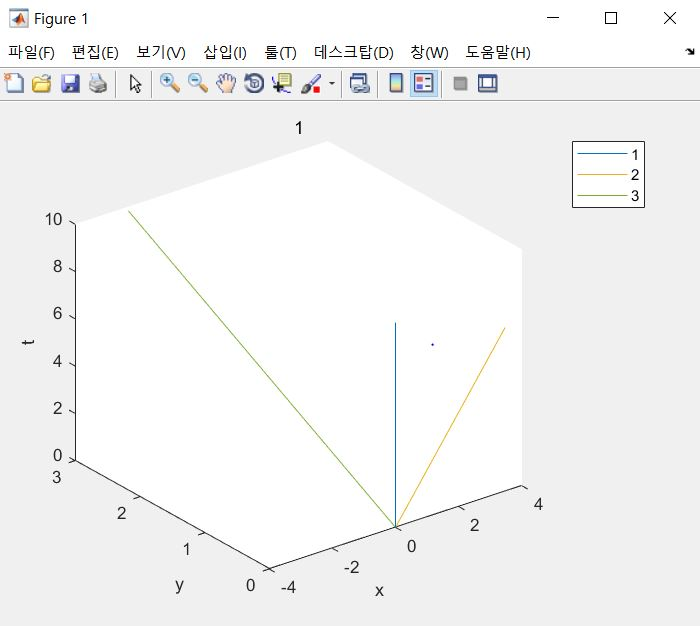
\includegraphics[width=0.7\linewidth]{images/figure}
	\caption{민코스프키 시공도식}
	\label{fig:figure}
\end{figure}

\begin{figure}[h]
	\centering
	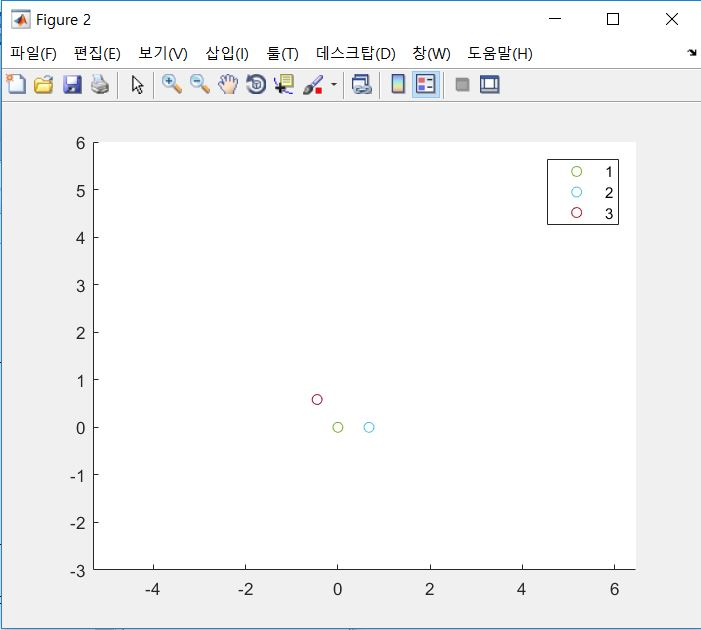
\includegraphics[width=0.7\linewidth]{images/animation}
	\caption{애니메이션}
	\label{fig:animation}
\end{figure}

\lstset{language=Matlab,%
	%basicstyle=\color{red},
	breaklines=true,%
	morekeywords={matlab2tikz},
	keywordstyle=\color{blue},%
	morekeywords=[2]{1}, keywordstyle=[2]{\color{black}},
	identifierstyle=\color{black},%
	stringstyle=\color{mylilas},
	commentstyle=\color{mygreen},%
	showstringspaces=false,%without this there will be a symbol in the places where there is a space
	numbers=left,%
	numberstyle={\tiny \color{black}},% size of the numbers
	numbersep=9pt, % this defines how far the numbers are from the text
	emph=[1]{for,end,break},emphstyle=[1]\color{red}, %some words to emphasise
	%emph=[2]{word1,word2}, emphstyle=[2]{style},    
}


\lstinputlisting{main.m}

\subsection{GUI 프로그램}
Text 기반 시뮬레이션 프로그램을 참조하여, MATLAB의 GUI 제작 프로그램을 활용하여 GUI 프로그램을 제작하였다. 해당 프로그램의 작동 모습은 다음과 같다.

\begin{figure}
	\centering
	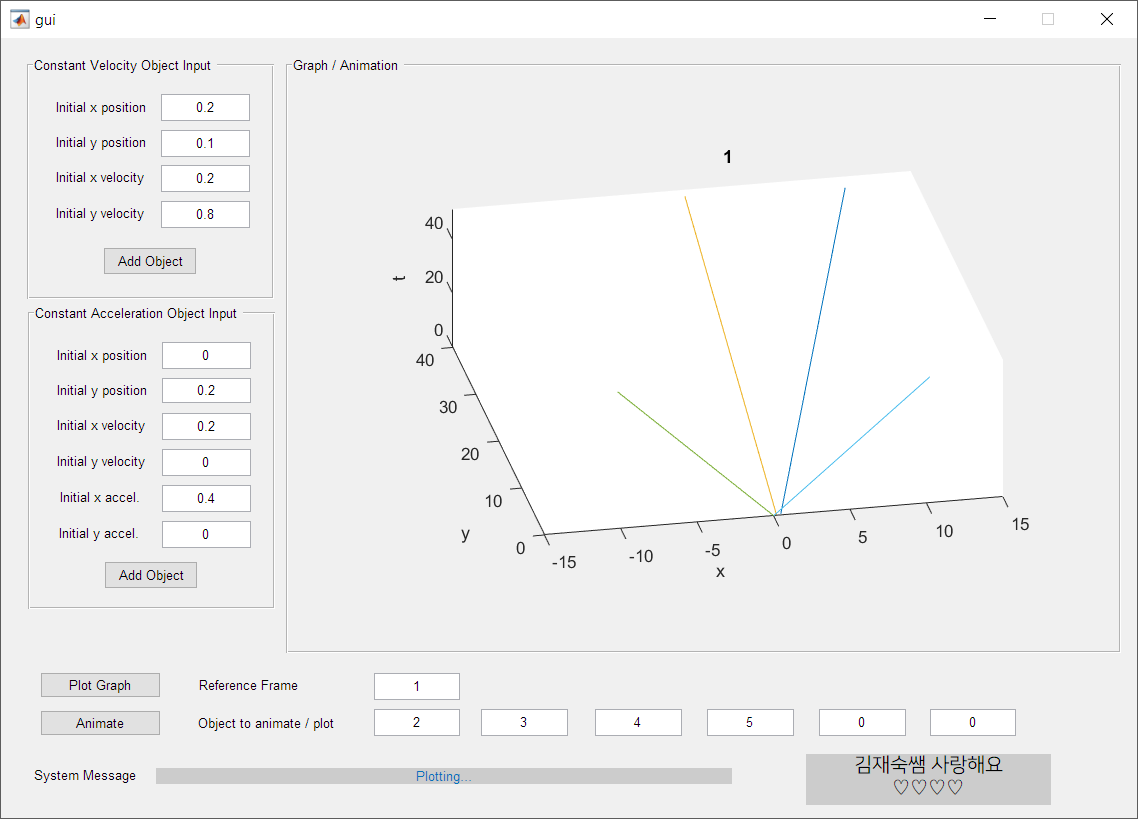
\includegraphics[width=0.8\linewidth]{images/gui}
	\caption{GUI 프로그램}
	\label{fig:gui}
\end{figure}

\chapter{결론}
본 연구에서는 특수상대성이론을 선형변환으로 해석하여, R Tilde 행렬이라는 쌍곡삼각함수로 이루어진 회전 행렬에 대하여 탐구해 보았다. 그 결과 R Tilde 행렬은 오일러 회전 행렬과 여러 가지 공통점을 가지고 있었으며, 이는 다양한 이차곡선의 변환에서도 드러났다.

한편 본 연구에서는 MATLAB을 이용하여 특수상대성이론에서 일어나는 많은 현상을 시뮬레이션 할 수 있는 프로그램을 제작하였다. 이 과정에서 R Tilde 행렬을 이용하여 일반적인 경우에 적용할 수 있는 로렌츠 변환 행렬을 만들어내었다. 제작 결과 등속도 혹은 약간의 가속도를 가진 물체들이 관성계에서 어떻게 보이는 지 민코프스키 시공도식을 그리고 애니메이션을 제작하였다.

본 연구의 가치는 직관적으로 받아들이기 어려운 특수 상대성이론에 대해 다양한 경우를 테스트할 수 있는 시뮬레이션 프로그램을 개발하였다는 데에 그 의의가 있다. 또한 이 과정에서 MATLAB에게 특화되어 있는 행렬 연산을 위해 로렌츠 변환 행렬을 일반적인 경우에 대하여 제작하였으며, 이 과정에서 R Tilde 행렬의 다양한 수학적인 성질을 알아보았다는 의의도 있다.
\newpage
\begin{thebibliography}{10}
	\bibitem{1}
	Schutz, A First Course in General Relativity
	
	\bibitem{2}
	\href{http://novicemathandscience.blogspot.com/2012/04/hermann-german.html}{Novice Math and Science:}
	
	\bibitem{3}
	\href{https://en.wikipedia.org/wiki/Minkowski_diagram
	}{Minkowski Spacetime Diagram Wikipedia}
	
	\bibitem{4}
	Khan Academy: 	Lecture on Minkowski Spacetime Diagram 
	and Derivations of Lorentz Transformation
	
	\bibitem{5}
	S.Friedberg, A.Insel, L.Spence, Linear Algebra
	
	
\end{thebibliography}
\end{document}